\documentclass{article}
\usepackage{amsmath} % import of math elements
%\usepackage{mathtools} %import of other math elements
\usepackage{tikz} 
\usetikzlibrary{shapes,positioning,calc} 
\usetikzlibrary{positioning,matrix, arrows.meta}
\usetikzlibrary{decorations.pathreplacing}
\usepackage{listings}
\usepackage{color}
\definecolor{dkgreen}{rgb}{0,0.6,0}
\definecolor{gray}{rgb}{0.5,0.5,0.5}
\definecolor{mauve}{rgb}{0.58,0,0.82}

\lstset{frame=tb,
  language=Bash,
  aboveskip=3mm,
  belowskip=3mm,
  showstringspaces=false,
  columns=flexible,
  basicstyle={\small\ttfamily},
  numbers=none,
  numberstyle=\tiny\color{gray},
  keywordstyle=\color{blue},
  commentstyle=\color{dkgreen},
  stringstyle=\color{mauve},
  breaklines=true,
  breakatwhitespace=true,
  tabsize=3
}

%-------------------------------------------------------
% Document information
%-------------------------------------------------------

\title{Algorithm and data structures} %Title 

\author{Roberto \textsc{Antoniello}} %author name

\begin{document}
\maketitle % show the title and author and date
%-------------------------------------------------------
%Introduction
%-------------------------------------------------------

\begin{center} In this file I will resume all the concepts I liked while studying the course of Algorithm and data structures.\end{center}

\section{Binary search}
This algorithm can be used only if you have a sorted array. Here how it works: \\
BinarySearch take a sorted array as input and return an index as output. So it returns the index of the found element or -1 if not found.\\
When it starts execution, the algorithm saves three variables sx, dx and m. The "m" variable is the index in the middle of the array, sx and dx are the first and the last index. It asks if the element is less or more than the element in m position. \\
Basically, if the element is x the question is: 
x $<$ A[m]  or  x $>$ A[m] ? 
We are reducing the search space by 2 every time because if it's less, our "dx" becomes "m", otherwise our "sx" becomes "m+1". \\
At the first iteration the search space is n elements, at the second it is $\cfrac{n}{2}$, at the third one it is $\cfrac{n}{2^2}$ and so on.\\
At the i° iteration it will be $\cfrac{n}{2^i}$.\\
During the last iteration the size of our array A is 1. So:\\
$\cfrac{n}{2^i} = 1 \Rightarrow n = 2^i \Rightarrow i = \log_2{n}$ \\
We have just said the amount of steps are $\log_2{n} \Rightarrow O(\log{n})$ \\
Here below there's an array as example with the initial value of sx,m and dx. \\

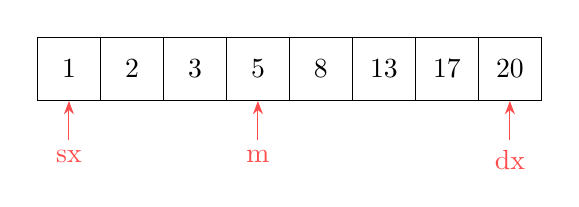
\begin{tikzpicture}
    \matrix (A) [matrix of nodes, nodes={draw, minimum size=8mm},
    column sep=-\pgflinewidth]{
        1 & 2 & 3 & 5 & 8 & 13 & 17 & 20\\
    };

    \foreach \i [evaluate=\i as \ni using {int(\i)},] in {1, 4, 8}{
        \pgfmathtruncatemacro{\half}{(\i + 1) / 2}
        \ifnum \i = 1
            \def\arrowlabel{sx}
        \else
            \ifnum \i = 4
                \def\arrowlabel{m}
            \else
                \def\arrowlabel{dx}
            \fi
        \fi
        \draw [{Stealth}-, red!70] (A-1-\ni.south) -- ++(-90:5mm) node[below] {\arrowlabel};
    }
\end{tikzpicture}

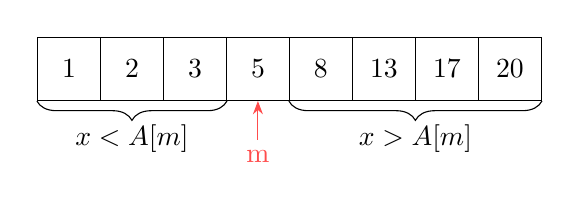
\begin{tikzpicture}
    \matrix (A) [matrix of nodes, nodes={draw, minimum size=8mm},
    column sep=-\pgflinewidth]{
        1 & 2 & 3 & 5 & 8 & 13 & 17 & 20\\
    };

    \foreach \i [evaluate=\i as \ni using {int(\i)},] in {4}{
        \pgfmathtruncatemacro{\half}{(\i + 1) / 2}
        \ifnum \i = 4
        		\def\arrowlabel{m}
        	\fi
        \draw [{Stealth}-, red!70] (A-1-\ni.south) -- ++(-90:5mm) node[below] {\arrowlabel};
    }

    % Brace for x < A[m]
    \draw [decorate,decoration={brace,amplitude=7pt,mirror},xshift=-1pt,yshift=-2pt]
        (A-1-1.south west) -- (A-1-3.south east) node[midway,below=5pt] {${x < A[m]}$};

    % Brace for x > A[m]
    \draw [decorate,decoration={brace,amplitude=7pt,mirror},xshift=-1pt,yshift=-2pt]
        (A-1-5.south west) -- (A-1-8.south east) node[midway,below=5pt] {${x > A[m]}$};
\end{tikzpicture}


I let you read the pseudocode here below. \\ \\ \\

\begin{lstlisting}[caption={\\\textit{Iterative version of the binary search algorithm.}}]
Algorithm BinarySearch(Array A[0,..,n-1]) --> index
	sx <-- 0
	dx <-- n
	index <-- -1
	while sx < dx do
		m <-- (sx+dx) / 2
		if x < A[m] then
			dx <-- m
		else if x = A[m] then
			index <-- m
		else
			sx <-- m+1
\end{lstlisting}

\section{Selection Sort}


\end{document}
